\documentclass[tikz,border=5mm]{standalone}
\usepackage{xcolor}
\usetikzlibrary{decorations.markings, arrows.meta}

\definecolor{gamegreen}{RGB}{58, 107, 34}

\begin{document}
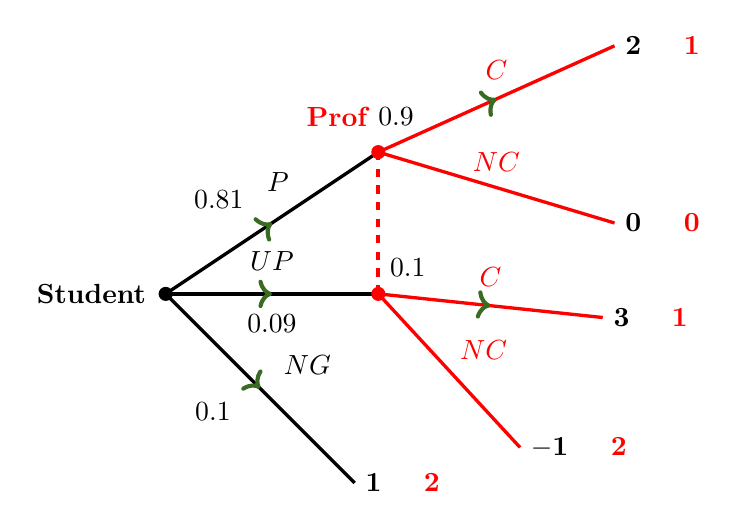
\begin{tikzpicture}[
    scale=1.5,
    font=\bfseries,
    dot/.style={circle, fill=#1, inner sep=1.8pt},
    dot/.default=black,
    line width=1.2pt,
    % Style to put a green arrow along the branch
    green arrow/.style={
        postaction={
            decorate,
            decoration={
                markings,
                mark=at position 0.5 with {
                    \arrow[gamegreen, line width=1.5pt]{>};
                }
            }
        }
    }
]

    % Coordinates
    \coordinate (root)    at (0, 0);
    \coordinate (qg_top)  at (1.8, 1.2);
    \coordinate (qg_mid)  at (1.8, 0);
    \coordinate (leaf_ng) at (1.6, -1.6);
    
    \coordinate (leaf1) at (3.8, 2.1);
    \coordinate (leaf2) at (3.8, 0.6);
    \coordinate (leaf3) at (3.7, -0.2);
    \coordinate (leaf4) at (3.0, -1.3);

    % Level 1 branches (You - Black)
    \draw[black, green arrow] (root) -- (qg_top);
    \node at (0.45, 0.8) {$0.81$};
    \node at (0.95, 0.95) {$P$};

    \draw[black, green arrow] (root) -- (qg_mid);
    \node at (0.9, 0.28) {$UP$};
    \node at (0.9, -0.25) {$0.09$};

    \draw[black, green arrow] (root) -- (leaf_ng);
    \node at (1.2, -0.6) {$NG$};
    \node at (0.4, -1.0) {$0.1$};

    % Information Set (Dashed Red Line)
    \draw[red, dashed, line width=1.5pt] (qg_top) -- (qg_mid);

    % Level 2 branches (QG - Red)
    \draw[red, green arrow] (qg_top) -- (leaf1) node[midway, above=3pt] {$C$};
    \draw[red] (qg_top) -- (leaf2) node[midway, above=2pt] {$NC$};
    
    \draw[red, green arrow] (qg_mid) -- (leaf3) node[midway, above=3pt] {$C$};
    \draw[red] (qg_mid) -- (leaf4) node[midway, above right] {$NC$};

    % Nodes & Labels
    \node[dot=black, label=left:Student] at (root) {};
    \node[dot=red] at (qg_top) {};
    \node[dot=red] at (qg_mid) {};

    % Un-overlapped labels for QG and beliefs (0.9, 0.1)
    \node[red]   at (1.45, 1.5) {Prof};
    \node[black] at (1.95, 1.5) {$0.9$};
    \node[black] at (2.05, 0.22) {$0.1$};

    % Payoffs (You: black, QG: red)
    \node[right] at (leaf1) {2 \quad \textcolor{red}{1}};
    \node[right] at (leaf2) {0 \quad \textcolor{red}{0}};
    \node[right] at (leaf3) {3 \quad \textcolor{red}{1}};
    \node[right] at (leaf4) {$-$1 \quad \textcolor{red}{2}};
    \node[right] at (leaf_ng) {1 \quad \textcolor{red}{2}};

\end{tikzpicture}
\end{document}
